\chapter{先天免疫}\label{ch:g12:innate-immunity}

一根木刺扎进指尖，一分钟之内就被拔了出来。
到了傍晚，伤处发红、发热、肿胀、搏动性疼痛；次日，
皮下已形成一颗黄色的脓点；到第三天，
这些症状便消失了。这一过程中无任何“决定”，也无任何“学习”：同样的四种症状
出现在每一处伤口、每一个人、每一种哺乳动物身上，而且
早在人们知道木刺携带细菌之前就已如此。它们是
人体第一道防线的外在表现——一组\omterm{def:g10:cells-common-unit:cell}{细胞}
和分子，它们能在几分钟内识别入侵者并加以攻击，
即便从未与之接触过。本章描述这道防线；下一章
将描述它所调动的、较慢的、具有学习能力的防御。

\section{两种免疫}

\begin{definition}[先天免疫与适应性免疫]\label{def:g12:innate-immunity:immunity}
\emph{免疫系统}\index{免疫系统}是指由器官、
\omterm{def:g10:cells-common-unit:cell}{细胞}和分子组成的集合，用于抵御感染和
损伤。它分为两部分。\emph{先天免疫}\index{先天免疫}
自出生起即存在，在数分钟至数小时内发挥作用，能识别大类
入侵者——细菌、病毒、真菌、受损\omterm{def:g10:cells-common-unit:cell}{细胞}——所共有的
特征，且每次的应答方式都相同。
\emph{适应性免疫}\index{适应性免疫}需要数天才能起效，
能逐一识别每种入侵者，并对其形成记忆
（见\cref{ch:g12:adaptive-immunity}）。先天免疫系统为所有
动物所共有；适应性免疫仅存在于\omterm{def:g10:common-ancestry:bodyplan}{脊椎动物}中，且其启动
依赖于先天免疫。
\end{definition}

\begin{proposition}[屏障优先]\label{prop:g12:innate-immunity:barriers}
绝大多数入侵者根本无法进入体内。皮肤干燥、呈酸性，并不断脱落其
表层，几乎能阻挡一切；气道、消化道和生殖道的
内壁虽然潮湿，却覆有黏液，黏液能捕获微生物，
并随之被清除或得以更新；泪液、唾液和黏液
中都含有能分解细菌\omterm{def:g10:cells-common-unit:organelle}{细胞壁}的酶；胃酸以及
占据空间的肠道自身细菌，使新来者难有立足之地。
本章所述的免疫应答始于屏障
被突破之时。
\end{proposition}
\admitted

\section{炎症反应}

\begin{proposition}[四种症状及其成因]\label{prop:g12:innate-immunity:inflammation}
屏障被突破——伤口、感染、烧伤——会在数分钟内引发
\emph{炎症反应}\index{炎症反应}：发红、发热、
肿胀和疼痛。每种症状都有其成因：
\begin{itemize}
  \item \emph{哨兵\omterm{def:g10:cells-common-unit:cell}{细胞}}驻留于组织中，包括巨噬\omterm{def:g10:cells-common-unit:cell}{细胞}、
        \omterm{prop:g12:innate-immunity:handover}{树突状细胞}和肥大\omterm{def:g10:cells-common-unit:cell}{细胞}，它们带有受体，能识别
        整类微生物所共有的分子（如细菌\omterm{def:g10:cells-common-unit:organelle}{细胞壁}片段、病毒\omterm{def:g10:chemistry-of-life:families}{核酸}），
        以及受损\omterm{def:g10:cells-common-unit:cell}{细胞}释放的分子。识别之后，
        它们释放
        \emph{介质}\index{介质}：组胺、
        前列腺素，以及称为\omterm{def:g10:cells-common-unit:cell}{细胞}因子的信号蛋白。
  \item \omterm{prop:g12:innate-immunity:inflammation}{介质}使局部血管扩张，血管壁变得通透：
        血流量增加（引起发红、发热），血浆渗入
        组织（引起肿胀）。\omterm{prop:g12:innate-immunity:inflammation}{介质}还使神经末梢敏感
        （引起疼痛），并使血管壁变黏，
        便于经过的白\omterm{def:g10:cells-common-unit:cell}{细胞}附着。
  \item \emph{\omterm{def:g12:innate-immunity:phagocytosis}{吞噬细胞}}——血液中的中性粒\omterm{def:g10:cells-common-unit:cell}{细胞}在数小时内到达，
        单核\omterm{def:g10:cells-common-unit:cell}{细胞}则在一天之内转化为巨噬\omterm{def:g10:cells-common-unit:cell}{细胞}，穿出
        血管壁，沿\omterm{prop:g12:innate-immunity:inflammation}{介质}梯度爬行至
        损伤部位，吞噬并消化微生物和碎屑。
        死亡的\omterm{def:g12:innate-immunity:phagocytosis}{吞噬细胞}、细菌和液体即为脓液。
\end{itemize}
这一应答局部、迅速，对木刺与对细菌的反应相同：
它无需事先与入侵者接触。
\end{proposition}
\begin{proof}[证据]
仅将细菌\omterm{def:g10:cells-common-unit:organelle}{细胞壁}片段注入皮下，而不含
任何活菌，一小时内即可引发完整的应答：其
信号是分子模式，而非微生物本身。
阻断组胺（借助治疗花粉热的抗组胺药），可消除早期的发红和
肿胀；阻断合成前列腺素的酶（使用阿司匹林
或布洛芬），可减轻肿胀、疼痛和发热。
在显微镜下观察伤口可见，中性粒\omterm{def:g10:cells-common-unit:cell}{细胞}沿血管壁
滚动、停驻、穿过血管壁，并在两小时内聚集到
损伤部位；中性粒\omterm{def:g10:cells-common-unit:cell}{细胞}被清除的小鼠，会死于
正常小鼠一夜之内即可清除的感染。
\end{proof}

\begin{omfigure}
\begin{tikzpicture}[font=\small, >=Stealth,
  b/.style={draw, rounded corners, align=center, text width=2.5cm, minimum height=1.1cm}]
  \node[b, fill=omThm!12] (breach) at (0,0) {破损：伤口，\\ 细菌侵入};
  \node[b, fill=omProp!15] (sent) at (3.3,0) {哨兵细胞 \\ 识别 \\ 微生物模式};
  \node[b, fill=omProp!15] (med) at (6.6,0) {释放介质：\\ 组胺、\\ 前列腺素、细胞因子};
  \node[b, fill=omDef!12] (ves) at (9.9,1.4) {血管扩张 \\ 并渗漏：发红、\\ 发热、肿胀};
  \node[b, fill=omDef!12] (nerve) at (9.9,-1.4) {神经末梢 \\ 敏化：疼痛};
  \node[b, fill=omMeth!15, text width=2.8cm] (phag) at (13.4,0) {吞噬细胞离开 \\ 血液，吞噬 \\ 微生物：脓液};
  \draw[->, thick] (breach) -- (sent); \draw[->, thick] (sent) -- (med);
  \draw[->, thick] (med) -- (ves); \draw[->, thick] (med) -- (nerve);
  \draw[->, thick] (ves) -- (phag);
\end{tikzpicture}

{\small 按顺序展示\omterm{prop:g12:innate-immunity:inflammation}{炎症反应}。哨兵\omterm{def:g10:cells-common-unit:cell}{细胞}借助分子模式探测
入侵者并释放\omterm{prop:g12:innate-immunity:inflammation}{介质}；\omterm{prop:g12:innate-immunity:inflammation}{介质}
作用于血管和神经，引发四种症状，并
召集清除损伤部位的\omterm{def:g12:innate-immunity:phagocytosis}{吞噬细胞}。}
\end{omfigure}

\begin{omfigure}
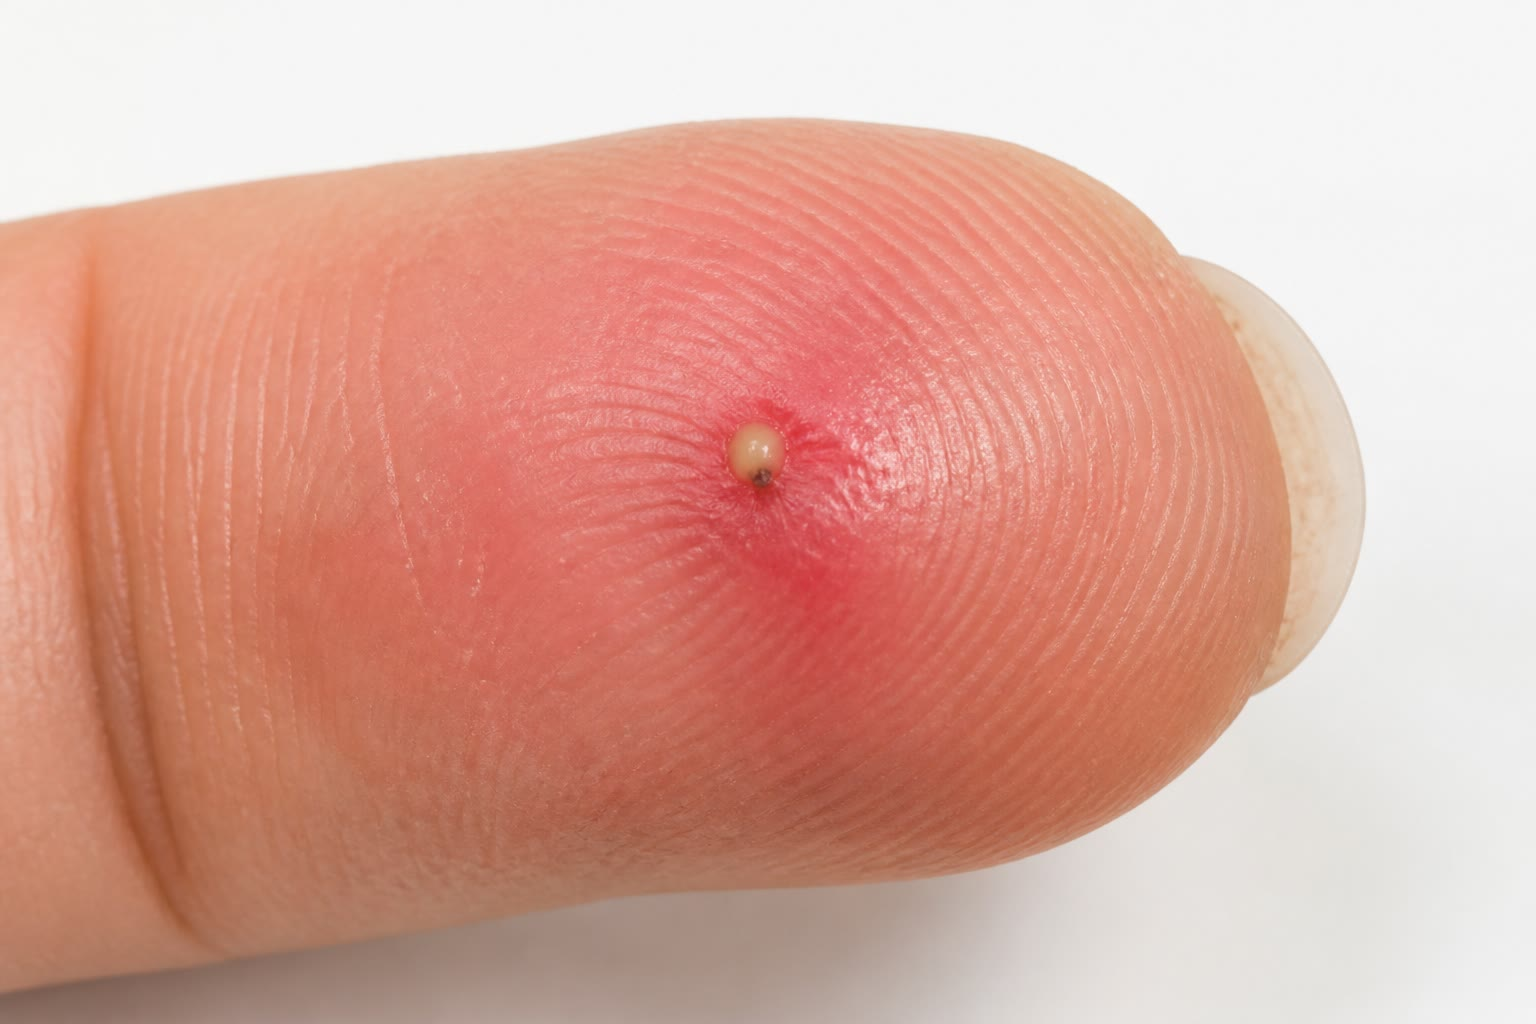
\includegraphics[width=0.56\linewidth]{images/book2/ai/g12-innate-inflamed-finger.jpg}

{\small 次日的木刺伤口：发红、肿胀、疼痛，入口处有一颗
脓点，即\omterm{prop:g12:innate-immunity:inflammation}{炎症反应}的外在表现。
脓液即前来作战并死亡的\omterm{def:g12:innate-immunity:phagocytosis}{吞噬细胞}。}
\end{omfigure}

\begin{definition}[吞噬作用]\label{def:g12:innate-immunity:phagocytosis}
\emph{吞噬作用}\index{吞噬作用}是指\omterm{def:g10:cells-common-unit:cell}{细胞}吞入一个颗粒的过程，
颗粒可以是细菌、死亡\omterm{def:g10:cells-common-unit:cell}{细胞}或一粒尘埃——
即\omterm{def:g10:cells-common-unit:cell}{细胞}以\omterm{def:g10:cells-common-unit:cell}{细胞}膜将其包裹，以囊泡形式将其拉入胞内，
再用酶和活性化学物质将其消化。\omterm{def:g12:innate-immunity:immunity}{先天免疫}反应中的
\emph{吞噬细胞}\index{吞噬细胞}主要是中性粒\omterm{def:g10:cells-common-unit:cell}{细胞}和巨噬\omterm{def:g10:cells-common-unit:cell}{细胞}：
前者寿命短、数量多，后者寿命长，
常驻于组织中。巨噬\omterm{def:g10:cells-common-unit:cell}{细胞}消化掉一个微生物后，
会保留其\omterm{def:g11:gene-expression:protein}{蛋白质}的片段，并将其展示于\omterm{def:g10:cells-common-unit:cell}{细胞}表面——
这一步将本反应与下一章的内容联系起来。
\end{definition}

\begin{omfigure}
\begin{tikzpicture}[font=\small, >=Stealth, line cap=round]
  \tikzset{ph/.style={draw, thick, fill=omDef!12}}
  % 1 contact
  \draw[ph] (0,0) circle (1.0); \draw[thick, fill=omThm!40, rounded corners=3pt] (1.05,-0.15) rectangle (1.75,0.15);
  \node[anchor=north, align=center] at (0.5,-1.2) {1. 接触：\\ 受体结合微生物};
  % 2 engulfing
  \begin{scope}[xshift=4.2cm]
    \draw[ph] (0,0) circle (1.0);
    \draw[thick, omDef!80!black, fill=omDef!12] (0.55,0.7) .. controls (1.5,0.6) and (1.5,-0.6) .. (0.55,-0.7);
    \draw[thick, fill=omThm!40, rounded corners=3pt] (0.75,-0.15) rectangle (1.35,0.15);
    \node[anchor=north, align=center] at (0.5,-1.2) {2. 包裹：\\ 细胞膜将其包住};
  \end{scope}
  % 3 vesicle + digestion
  \begin{scope}[xshift=8.4cm]
    \draw[ph] (0,0) circle (1.0);
    \draw[thick, fill=white] (0.1,0.1) circle (0.42);
    \draw[thick, fill=omThm!40, rounded corners=2pt] (-0.15,0.0) rectangle (0.35,0.2);
    \foreach \a in {30,100,170,240,310} \fill[omProp] (\a:0.6) circle (1.5pt);
    \node[anchor=north, align=center] at (0,-1.2) {3. 囊泡内消化};
  \end{scope}
  % 4 display
  \begin{scope}[xshift=12.2cm]
    \draw[ph] (0,0) circle (1.0);
    \foreach \a in {60,120,200} { \draw[thick] (\a:1.0) -- (\a:1.35); \fill[omThm] (\a:1.4) circle (2pt); }
    \node[anchor=north, align=center] at (0,-1.2) {4. 片段 \\ 展示于表面};
  \end{scope}
\end{tikzpicture}

{\small \omterm{def:g12:innate-immunity:phagocytosis}{吞噬作用}。\omterm{def:g12:innate-immunity:phagocytosis}{吞噬细胞}与微生物结合，将其包入
膜中，在囊泡中将其消化；若为巨噬\omterm{def:g10:cells-common-unit:cell}{细胞}或
\omterm{prop:g12:innate-immunity:handover}{树突状细胞}，则将微生物\omterm{def:g11:gene-expression:protein}{蛋白质}的片段展示于其表面，
以供\omterm{def:g12:innate-immunity:immunity}{适应性免疫}的\omterm{def:g10:cells-common-unit:cell}{细胞}识别。}
\end{omfigure}

\begin{omfigure}
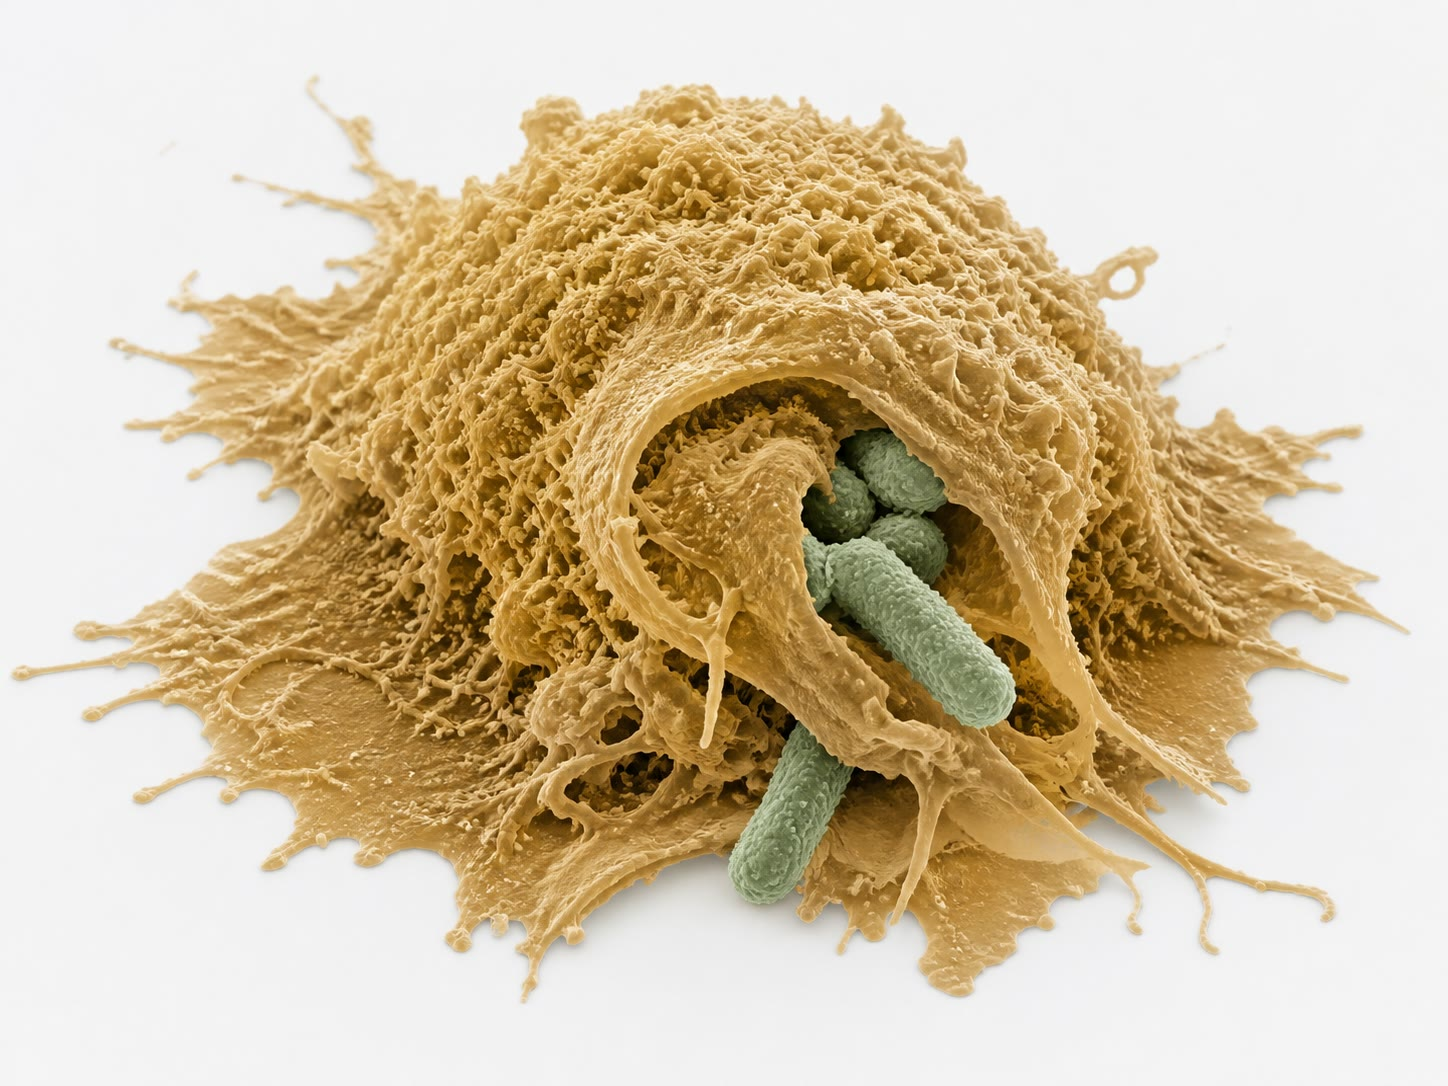
\includegraphics[width=0.56\linewidth]{images/book2/ai/g12-innate-macrophage-sem.jpg}

{\small 伪彩色电子显微照片中，一个巨噬\omterm{def:g10:cells-common-unit:cell}{细胞}
正伸展\omterm{def:g10:cells-common-unit:cell}{细胞}膜，包围即将吞入的细菌。
这是\omterm{def:g12:innate-immunity:immunity}{先天免疫}反应的主力\omterm{def:g10:cells-common-unit:cell}{细胞}。}
\end{omfigure}

\begin{example}[木刺的时间表]\label{ex:g12:innate-immunity:timetable}
0 分钟：细菌从木刺进入组织。1--10 分钟：
肥大\omterm{def:g10:cells-common-unit:cell}{细胞}和巨噬\omterm{def:g10:cells-common-unit:cell}{细胞}识别细菌壁的片段，释放
组胺和\omterm{def:g10:cells-common-unit:cell}{细胞}因子，血管扩张。1 小时：发红、发热，
第一批中性粒\omterm{def:g10:cells-common-unit:cell}{细胞}穿过血管壁。2--12 小时：中性粒\omterm{def:g10:cells-common-unit:cell}{细胞}
大量聚集，吞噬细菌后死亡；肿胀和疼痛达到高峰。1 天：
单核\omterm{def:g10:cells-common-unit:cell}{细胞}到达并转化为巨噬\omterm{def:g10:cells-common-unit:cell}{细胞}，清除碎片；可见脓液。
2--3 天：细菌已消失，\omterm{prop:g12:innate-immunity:inflammation}{介质}不再释放，血管恢复
正常，修复开始。若细菌增殖快于
\omterm{def:g12:innate-immunity:phagocytosis}{吞噬细胞}的清除，则反应范围扩大，出现发热，
\omterm{def:g12:innate-immunity:immunity}{适应性免疫}反应——已在淋巴结中启动——便接替上场。
\end{example}

\section{平息反应}

\begin{proposition}[抗炎药]\label{prop:g12:innate-immunity:drugs}
\omterm{prop:g12:innate-immunity:inflammation}{炎症反应}既有用又有代价：肿胀和疼痛
是清除入侵者所付出的代价；反应过度时，
若反应错误地针对无害的花粉或机体自身的\omterm{def:g10:muscles-and-joints:joint}{关节}，
或持续时间过长，它本身也会造成损伤。
\emph{抗炎药}\index{抗炎药}作用于炎症\omterm{prop:g12:innate-immunity:inflammation}{介质}：阿司匹林、
布洛芬及其同类药物可阻断合成前列腺素的酶，
从而减轻疼痛、肿胀和发热；皮质类固醇
由肾上腺\omterm{def:g11:hormones-and-reproduction:hormone}{激素}衍生而来，可抑制大多数\omterm{prop:g12:innate-immunity:inflammation}{介质}的生成，
用于严重或慢性炎症。所有药物都只能缓解症状，
无法消除病因。由于抑制了反应，
它们也可能延缓对真正感染的清除。
\end{proposition}
\admitted

\begin{omfigure}
\begin{tikzpicture}
\begin{axis}[
  width=0.86\linewidth, height=5.6cm,
  axis x line=bottom, axis y line=left,
  xmin=0, xmax=72, ymin=0, ymax=110,
  xlabel={受伤后时间（小时）}, ylabel={肿胀（占最大值的\%）},
  xlabel style={font=\small, at={(axis description cs:0.5,-0.12)}, anchor=north},
  ylabel style={font=\small},
  tick label style={font=\small}, xtick={0,12,24,36,48,60,72}, ytick={0,50,100},
  legend style={at={(0.97,0.95)}, anchor=north east, font=\small, draw=none},
  legend cell align=left,
]
\addplot[thick, omThm, smooth] coordinates {(0,0) (2,40) (6,85) (12,100) (24,80) (36,50) (48,25) (60,10) (72,3)};
\addplot[thick, omDef, dashed, smooth] coordinates {(0,0) (2,25) (6,45) (12,55) (24,45) (36,30) (48,15) (60,6) (72,2)};
\legend{未治疗, 使用抗炎药}
\end{axis}
\end{tikzpicture}

{\small 扭伤后的肿胀，有无服用\omterm{prop:g12:innate-immunity:drugs}{抗炎药}的对比。
该药物通过阻断前列腺素使肿胀减半；反应的
进程及其病因均未改变。}
\end{omfigure}

\begin{example}[发热]\label{ex:g12:innate-immunity:fever}
在大面积或持续性炎症部位释放的\omterm{def:g10:cells-common-unit:cell}{细胞}因子
到达脑部，使体温调定点升高，即发热。
体温升高一两度，可加快\omterm{def:g12:innate-immunity:phagocytosis}{吞噬细胞}的作用，抑制许多
细菌的生长，但要付出\omterm{def:g10:exercise-and-energy:expenditure}{能量消耗}和不适的代价；高于 \qty{40}{\celsius} 时，
代价超过收益，此时便使用解热药
（阻断前列腺素的药物）。发热是一种受调节的
反应，而非调节失灵。
\end{example}

\section{从先天免疫到适应性免疫}

\begin{proposition}[交接]\label{prop:g12:innate-immunity:handover}
在哨兵\omterm{def:g10:cells-common-unit:cell}{细胞}中，\emph{树突状细胞}\index{树突状细胞}
还承担第二项职能：吞下入侵者后，它们借淋巴管离开组织，
携带表面展示的入侵者蛋白片段，
前往最近的\emph{淋巴结}。在那里，
它们把这些片段呈递给\omterm{def:g12:innate-immunity:immunity}{适应性免疫}系统的淋巴\omterm{def:g10:cells-common-unit:cell}{细胞}，
所携带的\omterm{def:g10:cells-common-unit:cell}{细胞}因子告知这些淋巴\omterm{def:g10:cells-common-unit:cell}{细胞}入侵者的类型。
因此，\omterm{def:g12:innate-immunity:immunity}{先天免疫}反应不仅抵抗最初
数日的感染，还识别敌人并传递其特征。若无
这一交接，\omterm{def:g12:innate-immunity:immunity}{适应性免疫}反应便无从开始——因此疫苗
除抗原外，还含有能引发轻微
炎症的物质。
\end{proposition}
\admitted

\begin{omfigure}
\begin{tikzpicture}
\begin{axis}[
  width=0.86\linewidth, height=5.6cm,
  axis x line=bottom, axis y line=left,
  xmin=0, xmax=14, ymin=0, ymax=110,
  xlabel={感染后天数}, ylabel={反应强度（占最大值的 \%）},
  xlabel style={font=\small, at={(axis description cs:0.5,-0.12)}, anchor=north},
  ylabel style={font=\small},
  tick label style={font=\small}, xtick={0,2,4,6,8,10,12,14}, ytick={0,50,100},
  legend style={at={(0.5,-0.3)}, anchor=north, legend columns=2, font=\small, draw=none},
]
\addplot[thick, omThm, smooth] coordinates {(0,0) (0.2,60) (0.5,100) (1,95) (2,80) (3,60) (4,40) (5,25) (7,10) (10,3) (14,0)};
\addplot[thick, omDef, smooth] coordinates {(0,0) (2,0) (3,3) (4,10) (5,25) (6,50) (7,75) (8,90) (9,100) (11,95) (14,80)};
\legend{先天免疫反应（病灶处的吞噬细胞）, 适应性免疫反应（血液中的抗体）}
\end{axis}
\end{tikzpicture}

{\small 对首次感染的两种反应。\omterm{def:g12:innate-immunity:immunity}{先天免疫}反应在
数小时内即达到全强度，守住防线；适应性反应，
由\omterm{prop:g12:innate-immunity:handover}{树突状细胞}的报告启动，需一周才能达到其
峰值——而且与前者不同，它会留下记忆。}
\end{omfigure}

\begin{method}[读懂炎症]\label{met:g12:innate-immunity:read}
\begin{enumerate}
  \item 指出破损处和可能的入侵者（或无入侵者的损伤，
        扭伤也会引起炎症）。
  \item 将每种体征归因于其\omterm{prop:g12:innate-immunity:inflammation}{介质}及血管变化：
        发红与发热归因于血管扩张，肿胀归因于血管渗漏，
        疼痛归因于神经敏化。
  \item 辨认各阶段出现的\omterm{def:g10:cells-common-unit:cell}{细胞}：先是哨兵\omterm{def:g10:cells-common-unit:cell}{细胞}，
        数小时内出现中性粒\omterm{def:g10:cells-common-unit:cell}{细胞}，一天内出现巨噬\omterm{def:g10:cells-common-unit:cell}{细胞}；脓液则是它们的
        残骸。
  \item 判断反应是否适度：局限且
        数日内消退（说明反应按预期运作），
        若伴随发热而扩散（说明感染占上风，需适应性反应），或针对
        无害或慢性的对象（
        需考虑抗炎治疗）。
\end{enumerate}
\end{method}

\begin{remark}[古老、迅速而迟钝]\label{rem:g12:innate-immunity:old}
\omterm{def:g12:innate-immunity:immunity}{先天免疫}不仅属于人类，也是海绵、昆虫和橡树的免疫，
模式识别受体与\omterm{def:g12:innate-immunity:phagocytosis}{吞噬细胞}比\omterm{def:g10:common-ancestry:bodyplan}{脊椎动物}
早数亿年出现。它之所以迅速，是因为
针对各类敌人预先做好了准备；它之所以迟钝，也是出于同一原因：
它分不清此细菌与彼细菌，也无法
改进。下一章的系统两者兼能——但须
待本系统先发出警报之后。
\end{remark}

\section{练习}

\begin{exercise}[$\star$]\label{exo:g12:innate-immunity:1}
比较\omterm{def:g12:innate-immunity:immunity}{先天免疫}与\omterm{def:g12:innate-immunity:immunity}{适应性免疫}的三点区别。
\end{exercise}

\begin{exercise}[$\star$]\label{exo:g12:innate-immunity:2}
列出炎症的四个体征，
以及每个体征背后对应的血管或神经变化。
\end{exercise}

\begin{exercise}[$\star$]\label{exo:g12:innate-immunity:3}
哨兵\omterm{def:g10:cells-common-unit:cell}{细胞}识别什么？又释放什么？
\end{exercise}

\begin{exercise}[$\star$]\label{exo:g12:innate-immunity:4}
用四个步骤描述\omterm{def:g12:innate-immunity:phagocytosis}{吞噬作用}。
\end{exercise}

\begin{exercise}[$\star$]\label{exo:g12:innate-immunity:5}
阿司匹林和布洛芬如何减轻炎症？它们不能
做什么？
\end{exercise}

\begin{exercise}[$\star\star$]\label{exo:g12:innate-immunity:6}
根据两种反应的图示，\omterm{def:g12:innate-immunity:immunity}{先天免疫}反应何时达到峰值，
适应性反应何时达到峰值，两条曲线在第几天相交？
\end{exercise}

\begin{exercise}[$\star\star$]\label{exo:g12:innate-immunity:7}
单独注射一段细菌\omterm{def:g10:cells-common-unit:organelle}{细胞壁}片段，即可引发完整的
\omterm{prop:g12:innate-immunity:inflammation}{炎症反应}。这说明了什么？若注射的是无菌生理盐水，
又会发生什么？
\end{exercise}

\begin{exercise}[$\star\star$]\label{exo:g12:innate-immunity:8}
脓液由什么构成？为什么它在伤口形成一天后才
出现，而非立即出现？
\end{exercise}

\begin{exercise}[$\star\star$]\label{exo:g12:innate-immunity:9}
解释为什么抗组胺药能缓解花粉症，却
对细菌感染的后期阶段毫无作用。
\end{exercise}

\begin{exercise}[$\star\star$]\label{exo:g12:innate-immunity:10}
根据肿胀图，比较 12 小时和 36 小时时用药与未用药的肿胀程度，
该药能否缩短反应过程？
\end{exercise}

\begin{exercise}[$\star\star$]\label{exo:g12:innate-immunity:11}
无伤口、无微生物的扭伤踝\omterm{def:g10:muscles-and-joints:joint}{关节}出现发红、发热、
肿胀和疼痛。解释是什么触发了哨兵\omterm{def:g10:cells-common-unit:cell}{细胞}。
\end{exercise}

\begin{exercise}[$\star\star\star$]\label{exo:g12:innate-immunity:12}
缺乏中性粒\omterm{def:g10:cells-common-unit:cell}{细胞}的小鼠死于感染，而正常小鼠
一夜之间即可清除这些感染；缺乏\omterm{def:g12:innate-immunity:immunity}{适应性免疫}的小鼠能够存活，但
数周后死于感染。解释这两组结果分别说明了
两种系统的作用与时间特点。
\end{exercise}

\begin{exercise}[$\star\star\star$]\label{exo:g12:innate-immunity:13}
解释为什么医生可能不给脓肿患者开\omterm{prop:g12:innate-immunity:drugs}{抗炎药}，
而给\omterm{def:g10:muscles-and-joints:joint}{关节}炎患者开此类药物，
请依据每种炎症的成因加以说明。
\end{exercise}

\begin{exercise}[$\star\star\star$]\label{exo:g12:innate-immunity:14}
解释为什么\omterm{def:g12:innate-immunity:immunity}{先天免疫}反应不能随反复感染而增强，
而\omterm{def:g12:innate-immunity:immunity}{适应性免疫}反应却能，请从各自识别之物的性质
加以解释。
\end{exercise}

\begin{exercise}[$\star\star\star$]\label{exo:g12:innate-immunity:15}
“炎症是一种疾病。”请用一段话讨论：何时它起治疗作用，
何时它本身就是疾病，以及由什么因素决定。
\end{exercise}

\section{问题：木刺的三天}

\begin{problem}[{周末问题——逐小时追踪一处伤口：
细胞计数、介质追踪、药物检验，以及
向淋巴结交接的时刻计时}]
\label{pb:g12:innate-immunity:1}
一根木刺将约 $\num{10000}$ 个细菌带入指尖，它们
每 40 分钟分裂一次。伤口一毫米范围内的组织中驻留着 200 个巨噬\omterm{def:g10:cells-common-unit:cell}{细胞}；
中性粒\omterm{def:g10:cells-common-unit:cell}{细胞}自血液中于 1 小时后开始到达，
速率为每小时 $\num{50000}$ 个，每个
中性粒\omterm{def:g10:cells-common-unit:cell}{细胞}在死亡前可吞噬约 20 个细菌。

\medskip
\noindent\textbf{第一部分——较量。}
\begin{enumerate}
  \item 若没有任何细菌被杀灭，2 小时后有多少细菌，
        4 小时后又有多少？
  \item 200 个巨噬\omterm{def:g10:cells-common-unit:cell}{细胞}每小时各吞噬约 5 个细菌。第一小时它们
        共清除多少个细菌，
        这能否阻止细菌增长？
  \item 自第 1 小时起中性粒\omterm{def:g10:cells-common-unit:cell}{细胞}开始到达，
        第一小时到达的中性粒\omterm{def:g10:cells-common-unit:cell}{细胞}共能清除多少个细菌？
  \item 将其与第 2 小时的细菌\omterm{def:g12:selection-drift-speciation:population}{种群}相比，
        谁占优势？
  \item 大约到第几小时伤口被清除？
        伤口部位还残留什么？
\end{enumerate}

\medskip
\noindent\textbf{第二部分——征象。}
\begin{enumerate}[resume]
  \item 将发红、发热、肿胀和疼痛各自归因于
        某种\omterm{prop:g12:innate-immunity:inflammation}{介质}，以及血管或神经的某种变化。
  \item 解释肿胀为何有利于中性粒\omterm{def:g10:cells-common-unit:cell}{细胞}，以及为何
        会引起疼痛。
  \item 指尖随每次心跳而搏动。请从血管扩张和
        肿胀组织中的压强加以解释。
  \item 一天后形成了一小团脓液。列出其所含成分。
  \item 第 3 天征象已消退。什么停止了
        \omterm{prop:g12:innate-immunity:inflammation}{介质}的释放？
\end{enumerate}

\medskip
\noindent\textbf{第三部分——药物。}
\begin{enumerate}[resume]
  \item 在第 1 小时服用抗组胺药，它能缓解哪些
        征象，哪些不能？
  \item 在第 6 小时服用布洛芬，它阻断的是哪种
        \omterm{prop:g12:innate-immunity:inflammation}{介质}？它能缓解哪些征象？
  \item 涂抹糖皮质\omterm{def:g11:hormones-and-reproduction:hormone}{激素}乳膏后，
        中性粒\omterm{def:g10:cells-common-unit:cell}{细胞}的募集会发生什么变化，感染会面临
        怎样的风险？
  \item 解释三种药物为何都不能缩短感染过程，
        其中哪一种可能延长感染过程。
  \item 患者还出现 \qty{38.5}{\celsius} 的发热。
        哪些分子引起了发热，发热的作用是什么？
\end{enumerate}

\medskip
\noindent\textbf{第四部分——报告。}
\begin{enumerate}[resume]
  \item 第 2 小时吞噬了细菌的\omterm{prop:g12:innate-immunity:handover}{树突状细胞}，于第 20 小时
        抵达肘部的淋巴结，并展示细菌片段。
        除片段外，它们还携带什么？它们向谁
        传递信息？
  \item 根据两种免疫反应的图示，
        需经过多少天，针对这些细菌的抗体才会大量产生？它们
        对此次木刺感染是否仍需要？
  \item 同样的细菌一个月后经由第二根木刺侵入，
        哪一种免疫反应在第二次时不同，
        哪一种相同？
  \item 一人天生缺乏有功能的中性粒\omterm{def:g10:cells-common-unit:cell}{细胞}，靠每日服用\omterm{def:g11:antibiotic-resistance:antibiotic}{抗生素}存活。
        解释\omterm{def:g11:antibiotic-resistance:antibiotic}{抗生素}替代了防御的哪一部分，
        以及哪一部分它们无法替代。
  \item 写出结果：\omterm{def:g12:innate-immunity:phagocytosis}{吞噬细胞}在第几小时
        超过细菌数量；四种征象各自背后的\omterm{prop:g12:innate-immunity:inflammation}{介质}，以及
        将信息带到淋巴结的\omterm{def:g10:cells-common-unit:cell}{细胞}。
\end{enumerate}
\end{problem}
